\documentclass{article}
\usepackage{graphicx}
\usepackage{float}
\usepackage{geometry}
\usepackage{tcolorbox}
\usepackage{amssymb}
\usepackage{wasysym}
\usepackage{subcaption}
\usepackage{booktabs}
\usepackage{bm}
\usepackage{enumitem}
\usepackage{booktabs}
\usepackage{hyperref}
\usepackage{tabularx} % Required for full-width tables
\usepackage{colortbl} % Required for coloring the table cells
\usepackage{xcolor}   % Required for defining colors




\renewcommand{\labelenumi}{\Roman{enumi}.}
\definecolor{lightgray}{gray}{0.9} % Define lightgray color
\geometry{left=0.8in,right=0.8in,top=0.8in,bottom=1in}

\title{Experiment 2: Experimentation \& Evaluation 2023}
\author{Giorgio Bonetto \& Raffaele Perri}
\date{\today}

\begin{document}
\maketitle
\section*{Abstact}
Short (120-130 words) summary of your entire report. Give the reader a quick idea of what you did and what the main findings were (if you prepare this report ahead of time, leave out the findings until after you finish the analysis).


\section{Introduction}
In the realm of natural language reading, studies have demonstrated that the use of explicit separators between words significantly enhances reading speed—individuals tend to read 20\% faster when such separators are employed. Whether this finding extends to the realm of source code, specifically in the context of composed identifiers, remains an intriguing question. Composed identifiers, featuring more than one word, are commonly used in programming languages, and their readability can impact code comprehension and maintenance.

The focus of this experiment is to investigate whether the observed speedup in reading with explicit separators holds true for composed identifiers in source code. We specifically aim to compare two common styles of composing identifiers: camelCase and kebab-case. CamelCase involves concatenating words together, capitalizing the beginning of each new word (e.g., moveSouth), while kebab-case uses hyphens as separators between words (e.g., move-south).

The motivation behind this study is to shed light on whether the choice of identifier style influences reading efficiency in the context of programming. To achieve this, a controlled experiment has been designed to measure participants' reading speed and accuracy when identifying composed identifiers in both camelCase and kebab-case styles.

This report details the experimental design, methodology, and results of the study, aiming to contribute valuable insights to the ongoing discussion on coding conventions and their impact on code readability. Through a combination of careful experimentation and statistical analysis, we aim to answer the question: Does the choice of identifier style affect the speed and accuracy of code reading?



\begin{tcolorbox}[title=Hypothesis]
    Our hypothesis for this experiment is that the familiarity of participants with coding styles, specifically "camelCase" and "kebab-case," will significantly impact their accuracy in identifying and selecting the correct words in code snippets. We anticipate that participants familiar with both coding styles will demonstrate higher accuracy compared to those less familiar.
\end{tcolorbox}



\section{Method}
The method involves conducting a series of experiments where participants interact with code snippets containing words in camelCase or kebab-case. Demographic information is collected before starting the experiments. The participant's choices, correctness, and timing are recorded. The experiment progresses through a set number of trials, and data is submitted for each trial. After completing all experiments, the data is exported to a CSV file. The timing and correctness of responses are key variables of interest.
\subsection{Variables}

\begin{tcolorbox}[title=Independent Variables]

\textbf{Experiment Type (\texttt{currentCase}):}
\begin{itemize}
    \item \textbf{Description:} This variable represents the type of experiment being conducted, whether it's focused on camelCase or kebab-case.
    \item \textbf{Possible Values:} 'camelCase' or 'kebabCase'
\end{itemize}

\textbf{Participant Demographics (\texttt{participantData}):}
\begin{itemize}
    \item \textbf{Description:} Demographic information collected from the participant, including age, gender, programming experience, familiarity with camelCase, and familiarity with kebab-case.
    \item \textbf{Possible Values:} Various based on participant input.
\end{itemize}

\end{tcolorbox}

\begin{tcolorbox}[title=Dependent Variables]

\textbf{Word Selection (\texttt{boxWords}):}
\begin{itemize}
    \item \textbf{Description:} The set of words provided to the participant in each experiment, including the original word and the options in camelCase and kebab-case.
    \item \textbf{Possible Values:} Object containing word information.
\end{itemize}

\textbf{User Interaction and Responses:}
\begin{itemize}
    \item \textbf{Description:} The participant's interaction with the experiment, including clicking on words and the correctness of their choices.
    \item \textbf{Possible Values:} Clicked word, correctness (boolean), time taken.
\end{itemize}

\textbf{Experiment Counter (\texttt{counter}):}
\begin{itemize}
    \item \textbf{Description:} Keeps track of the current experiment number.
    \item \textbf{Possible Values:} Integer from 0 to the total number of experiments.
\end{itemize}

\end{tcolorbox}

\begin{tcolorbox}[title=Control Variables]

\textbf{Total Number of Experiments (\texttt{totalExperiments}):}
\begin{itemize}
    \item \textbf{Description:} Specifies the total number of experiments to be conducted.
    \item \textbf{Fixed Value:} 10 in this case.
\end{itemize}

\textbf{Starting Experiment State (\texttt{statingExperiment}):}
\begin{itemize}
    \item \textbf{Description:} Indicates whether the participant is in the personal information submission phase or the experiment phase.
    \item \textbf{Possible Values:} Boolean (true/false).
\end{itemize}

\end{tcolorbox}

\begin{tcolorbox}[title=Blocking Variables]

\textbf{Time-Related Variables (\texttt{startTime}, \texttt{endTime}, \texttt{timeTaken}):}
\begin{itemize}
    \item \textbf{Description:} Variables related to the timing of participant actions, including the start time, end time, and time taken to respond.
    \item \textbf{Possible Values:} Timestamps and duration in milliseconds.
\end{itemize}

\textbf{Experiment Routing (\texttt{\$router.push}):}
\begin{itemize}
    \item \textbf{Description:} The redirection of the participant to different experiment pages or the end view page.
    \item \textbf{Possible Values:} String (route name or path).
\end{itemize}

\textbf{Attempt Counter (\texttt{attempt}):}
\begin{itemize}
    \item \textbf{Description:} Keeps track of the number of attempts made by the participant in case of an incorrect response before advancing to the next word.
    \item \textbf{Possible Values:} Integer.
\end{itemize}

\end{tcolorbox}

\subsection{Design}
Check off the characteristics of your experimental design:\\

\textbf{Type of Study} (check one):\\
\noindent
\begin{minipage}{0.4\textwidth}
    \fbox{\Square{} \textbf{Observational Study}}
\end{minipage}%
\begin{minipage}{0.4\textwidth}
    \fbox{\bm{\XBox{}} \textbf{Quasi-Experiment}}
\end{minipage}%
\begin{minipage}{0.2\textwidth}
    \fbox{\Square{} \textbf{Experiment}}
\end{minipage}\\\\
The study follows a quasi-experimental design due to practical limitations in manipulating independent variables. Unlike a true experiment with complete control, this design prioritizes real-world conditions.

The experimenter controls the timing of dependent variable measurements but lacks control over participant assignment to different conditions. This compromise ensures a balance between external validity and limitations inherent in coding style familiarity research.

In summary, the quasi-experimental design allows for a nuanced exploration of coding style knowledge across diverse participants, striking a balance between controlled experiments and real-world complexities.
\\


\textbf{Number of Factors} (check one):\\
\noindent
\begin{minipage}{0.4\textwidth}
    \fbox{\Square\ \textbf{Single-Factor Design}}
\end{minipage}%
\begin{minipage}{0.4\textwidth}
    \fbox{\bm{\XBox{}} \textbf{Multi-Factor Design}}
\end{minipage}%
\begin{minipage}{0.0\textwidth}
    \fbox{\Square\ \textbf{Other}}
\end{minipage}\\\\
This experiment employs a Multi-factor Design, encompassing various independent variables to explore participants' responses to code snippets featuring both camelCase and kebab-case formats. The factors under examination include the coding style (randomly assigned as camelCase or kebab-case) and participants' familiarity with each style. These independent variables aim to uncover potential influences on participants' word recognition and selection. The study captures dependent variables, such as participants' responses (correct or incorrect) and the time taken for their selections. The randomized assignment of coding styles enhances the exploration of the interplay between coding style, familiarity, and participant responses within a Multi-factor Design framework:\\
\begin{figure}[H]
    \centering
    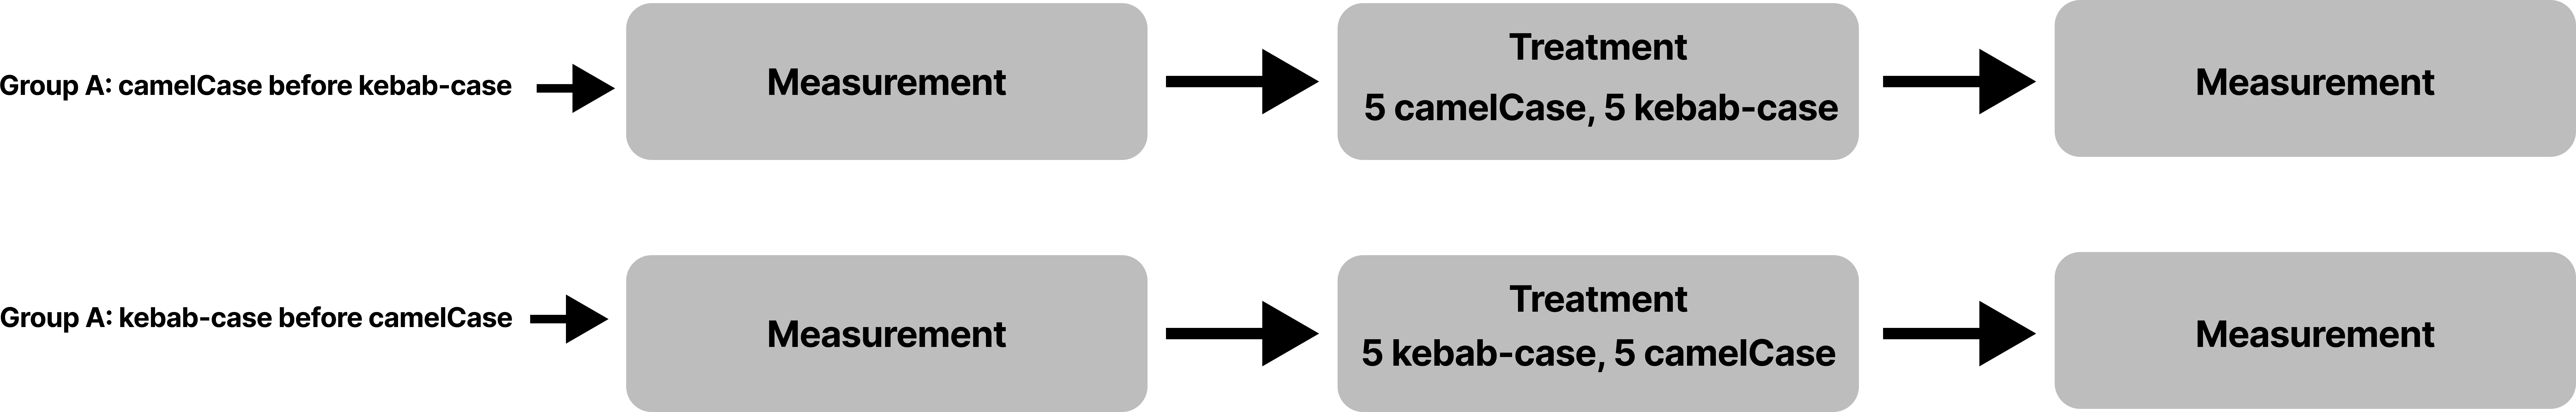
\includegraphics[width=1\textwidth]{graphExperiment2.png}
    \caption{Multi-factor design}
\end{figure}

\subsection{Participants}
Describe who will take / took part in your experiment. Provide descriptive/summative statistics of their gender, age, professional backgrounds, and any other characteristics that may be relevant to your experiment. Also explain how you will recruit / recruited them (volunteers recruited through email, classmates who were asked to do this, etc) and how you will allocate / allocated them into the different study conditions, i.e., control group vs experimental group(s).\textbf{TODO: THE GRAPHICAL PART AND INFORMATIONS ABOUT THE DEMOGRAPHICS}\\

The participants in this study encompass a diverse group of individuals, including students, professionals from various fields, and individuals with varying degrees of familiarity with informatics. The recruitment process involved approaching people in person, introducing the study, and inviting them to participate voluntarily.

\subsubsection*{Inclusion Criteria}

Participants were eligible to take part in the study if they:
\begin{itemize}
  \item Expressed willingness to engage in a simple test related to coding conventions.
  \item Represented a broad spectrum of backgrounds, including but not limited to students, non-technical professionals, and individuals with no specific informatics expertise.
\end{itemize}

\subsubsection*{Recruitment Process}

Recruitment was conducted in person, with us (researchers) approaching potential participants in various settings. These settings included educational institutions, public spaces, and community gatherings. The recruitment team provided a brief overview of the study, emphasizing its simplicity and the lack of specific informatics knowledge required.

\subsubsection*{Informed Consent}

Participants were informed about the nature of the study, its objectives, and the procedures involved. They were assured that participation was entirely voluntary and that they could withdraw from the study at any point without consequences. Informed consent was obtained from each participant before engaging in any experimental tasks.

\subsubsection*{Diversity Considerations}

Efforts were made to ensure diversity in the participant pool to capture a broad range of perspectives and experiences. This diversity contributes to the generalizability of findings and allows for a more comprehensive understanding of how individuals with different backgrounds approach coding conventions.

\subsubsection*{Confidentiality and Anonymity}

All collected data were treated with utmost confidentiality. Participants were assigned unique identifiers to protect their anonymity, and personal information was securely stored in compliance with data protection regulations.

\subsection{Apparatus and Materials}
Describe in sufficient detail any relevant “props” that you used in your experiment. This could be the computer
you used (exact model and specification), the software used (URL, version numbers), the way you measured, e.g.,
time (A stopwatch? A background process on the computer that got automatically triggered?). Omit needless
detail (e.g., think whether details like the size of the table the laptop was placed on, or the hard disk size, might
have affected your results or not)

\subsubsection*{Hardware}
The experiment was conducted using a \texttt{Dell Inc Precision 5550} laptop, featuring the following hardware specifications:
\begin{itemize}
  \item \textbf{Processor:} \texttt{Intel® Core™ i7-10850H × 12}
  \item \textbf{RAM:} (Specify the RAM capacity and type)
  \item \textbf{Storage:} (Specify the storage type and capacity)
  \item \textbf{Graphics:} (Specify the graphics card)
  \item \textbf{Display:} (Specify the display specifications)
  \item \textbf{Input Devices:} (Specify any additional input devices used, e.g., mouse, keyboard)
\end{itemize}

\subsubsection*{Software}
The software environment for the experiment was configured as follows:
\begin{itemize}
  \item \textbf{Operating System:} \texttt{Ubuntu 23.04} (64-bit)
  \item \textbf{Kernel Version:} \texttt{Linux 6.2.0-36-generic}
  \item \textbf{Firmware Version:} \texttt{1.24.1}
  \item \textbf{Programming Environment:} \texttt{VisualStudio Code, Intellij IDEA}
\end{itemize}

\subsubsection*{Measurement Tool}
    \begin{itemize}
      \item Utilized the \texttt{performance.now()} function for accurate measurement of execution time.
      \item Employed \texttt{Date.now()} for capturing program execution time.
      \item Used a digital stopwatch to cross-verify the time taken by the program.
    \end{itemize}

\subsubsection*{Experimental Setup}
Participants engaged with the experiment using the provided web application hosted on a local server. The application was accessed through a standard web browser (Google Chrome). The interaction with the experiment was carried out on the \texttt{Dell Inc.Precision 5550} laptop, ensuring a consistent hardware and software environment for all participants.

\subsubsection*{Data Collection Tools}
Data related to participant responses and interactions were collected using the Flask web framework on the server side. Additionally, client-side interactions were captured through the Vue.js framework in the web application. No personally identifiable information was collected, ensuring participant privacy and data confidentiality.

\subsubsection*{Randomization and Counterbalancing}
To minimize potential order effects, the order of presentation for experimental stimuli was randomized for each participant. This randomization was implemented using a custom script within the experimental software.

\subsubsection*{Control Measures}
The experiment was conducted in a controlled environment with minimal external distractions. Participants were provided with standardized instructions to ensure consistency in task execution. The web application interface was designed to be uniform across all sessions.


\subsection{Procedure}
Describe how you used your props and/or the participants to perform your actual experiment, i.e., how you actually carried out a single experimental run. What was done to the participants? What did they have to do? How long did each session take (unless this is an actual dependent variable)? If you did not have participants, explain, e.g., what software was started by whom in what order.\\\\
The experiment was conducted in a controlled environment following a standardized procedure. Participants were recruited through in-person interactions, where individuals from a diverse background, including students and those with no prior experience in informatics, were invited to participate in a simple coding style test.

\subsection*{Recruitment}

\begin{itemize}
  \item Participants were approached in person and asked if they would be interested in participating in a coding style test.
  \item The recruitment process involved individuals from various demographics, including students, professionals, and those with diverse interests.
  \item Participants were informed that the test aimed to assess their understanding of coding style conventions in different programming paradigms.
  \item Informed consent was obtained from each participant, emphasizing the voluntary nature of their participation and the confidentiality of their responses.
\end{itemize}

\subsection*{Personal Information Collection}

\begin{itemize}
  \item Participants who expressed interest were directed to a Personal Information View in the web application.
  \item Demographic information, including age, gender, programming experience, and familiarity with coding styles (camelCase and kebab-case), was collected through a structured form.
  \item The personal information collection process was designed to be brief and straightforward, ensuring a seamless transition to the experimental phase.
  \item After providing personal information, participants were guided through the experiment's instructions and purpose.
\end{itemize}

\subsection*{Experiment Instructions}

\begin{itemize}
  \item Participants were introduced to the coding style test, which consisted of 10 code snippets featuring both camelCase and kebab-case examples.
  \item Clear instructions were provided, explaining that each snippet contained clickable words, and participants were required to select the correct word based on coding style conventions.
  \item The experiment emphasized that the task was designed to assess participants' familiarity with coding styles rather than their coding proficiency.
\end{itemize}

\subsection*{Experiment Sessions}

\begin{itemize}
  \item The experiment was divided into two sessions, each featuring 5 code snippets. The order of camelCase and kebab-case snippets was randomized to mitigate order effects.
  \item Participants initiated the experiment by clicking the "Start" button, followed by a brief countdown to ensure readiness.
  \item During each session, participants clicked on words within code snippets, and the web application provided immediate feedback on the correctness of their choices.
  \item Incorrect selections required participants to click on the correct word before proceeding, reinforcing learning through corrective feedback.
\end{itemize}

\subsection*{Data Collection}

\begin{itemize}
  \item Throughout the experiment, participant interactions and responses were recorded, including selected words, response times, and correctness.
  \item After completing the coding style test, participants were directed to a debriefing page, thanking them for their participation and providing information about the study's objectives.
\end{itemize}

\subsection*{Export and Closure}

\begin{itemize}
  \item Participants were informed that their anonymized data would be used for research purposes only.
  \item The experiment concluded with the opportunity for participants to ask questions or seek additional information.
\end{itemize}

The entire procedure aimed to create a standardized and controlled environment for the coding style test while ensuring participant comfort and understanding.


\section{Results}
\subsection{Visual Overview}
Provide an insightful overview of the data you collected. This requires some engineering from your part, to find a good degree of summarization: On one end of the spectrum, you don't summarize, and report hundreds of raw measurement values in a block of text. On the other end of the spectrum, you report a single number (like a mean value). Both approaches are bad.

Instead, use appropriate visual summaries (such as scatter plots, histograms, box plots, or empirical cumulative distribution functions) to show the distribution of your data. If you have a very small number of measurement values, then report all of them in a well organized table (where rows and/or columns correspond to different levels of different factors).


\subsection{Descriptive Statistics}

For each group or condition, summarize the set of measured values with a "five-number summary": minimum, first quartile, median, third quartile, and maximum (note: these are the statistics underlying a box plot).

Moreover, report the mean and standard deviation (note: for data that is not normally distributed, e.g., for multi-modal data, these two statistics may be less meaningful).

Make sure you explain – in your words – what these statistics mean “in plain English”, but don’t yet interpret them (this is for the Discussion section).

\subsection{Inferential Statistics}
If applicable, you then follow these up with inferential statistics – i.e., the results of statistical tests that you did in order to decide whether there were any “real” (i.e., not by chance) differences between the conditions/groups. You should also explain what statistical test you used, and, if not immediately obvious, why.

Make sure you explain – in your words – what these statistics mean “in plain English”, but don’t yet interpret them (this is for the Discussion section).


\section{Discussion}
\subsection{Compare Hypothesis to Results}
Provide a brief restatement of the main results from the previous section, and if (or if not) these support your research hypothesis.

If there is a discrepancy between your hypothesis and the results of your experiment, speculate about why you were unable to find evidence to support your hypothesis.


\subsection{Limitations and Threats to Validity}Acknowledge any limitations and threats to validity of your study, and how seriously these affect your results. How could these be remedied in future work?

\subsection{Conclusions}

End with the main conclusions that can be drawn from your study.


\section{Appendix}
\subsection*{A. Materials}

Any documents you used for your informed consent (information sheets, consent) or as part of your apparatus (e.g., manual, hand-out), please include them here.

\subsection{Reproduction Package}

Before, during, and after the experiment you collected all kinds of data. Don't ever throw such data away! Any plots, tables, summaries, and statistics provided in this report should be recreatable from the raw data you have.

If you only collected a small amount of data, put it in this Appendix right here.

If you collected data in forms that are better kept in separate files, then zip up those files, and submit them as a "reproduction package" supporting this report.


\subsection*{{Github repo: (\url{https://github.com/Bonett0/experiment-02})}}




\end{document}
